\chapter{实验与评估}
\citestyle{ustcnumerical}

% \usepackage{graphicx}
% \usepackage{subfigure}

在本章中,由于OpenCL的多平台性,我们将在两个不同的平台上进行:一个是CPU上的并行计算,另一个是GPU上的并行计算。通过同样的一个OpenCL程序在两个不同的硬件架构上的运行来确定在不同的情况下各个在上一章中提到的常数,并用这些常数具体评估在不同硬件平台上的运行性能,并对这些结果进行对比。

\section{实验环境}
本次实验采取了两种并行硬件架构来完成实验:

1. 纯CPU架构运行在如下的硬件上:Intel Core i5 Dual Core Processor@2.9GHz,8GB 2133MHz LPDDR3 memory,512GB SSD。

2. CPU-GPU混合架构运行在如下的硬件上:ATI Radeon HD 8570, Intel Core i7-6700@3.4GHz(8 cores),8GB 2133MHz DDR3 memory, 128GB SSD

由于条件所限,实验时选择的GPU是相对较老的款式,性能上较为不足。因此实验数据的考察更偏向于对于相对并行性能的考察。另外,选择这块GPU的理由中也包括了基于“创造出一种条件,使得花费函数估计式中系数的比重有所不同”的考量。

\subsection{由实验环境进行的参数选择测试}
在进行实验之前,首先需要对上一章中提到的诸常数进行考察,从而明确在算法运行的全过程中哪方面将成为性能瓶颈。

对于$C_{copy\_hd\_to\_m}$:

对于$C_{copy\_hd\_to\_m}$的考察可以通过读取的文件的大小来确定。我们可以采用一个“纯粹的读取程序”——即只将数据读入内存,在读取的过程之中不进行任何多余的操作——来完成求出这个常量的实验。

因此,我们直接简单地利用现有程序中的“从硬盘中读入数据集”这一步来进行系数的计算。对不同大小的数据集进行读入所需要花费的时间为:(均为10次的平均数值)

在纯粹CPU架构上:
\begin{table}[!htbp]
\centering
\caption{纯CPU架构上的硬盘读写测试} 
\label{tab:table1}
\begin{tabular}{|c|c|c|}
    \hline
    数据条目数 & 总的数据集文件大小(byte) & 平均读取用时(s)\\
    \hline
    262144 & 3479769 & 0.3520096\\
    \hline
    2097152 & 27841394 & 2.741692\\
    \hline
    16777216 & 222741273 & 21.11312\\
    \hline
    134217728 & 1781907696 & 166.6692\\
    \hline
\end{tabular}
% \note{这里是表的注释}
\end{table}

取这四个数据点进行拟合,能得到直线的斜率,即我们所需的$C_{copy\_hd\_to\_m}$的估计值为$9.34613 \times 10^{-8}$s / byte

在CPU-GPU并行架构上:

\begin{table}[!htbp]
\centering
\caption{CPU-GPU架构上的硬盘读写测试} 
\label{tab:table2}
\begin{tabular}{|c|c|c|}
    \hline
    数据条目数 & 总的数据集文件大小(byte) & 平均读取用时(s)\\
    \hline
    262144 & 3479769 & 0.0813523\\
    \hline
    2097152 & 27841394 & 0.3875493\\
    \hline
    16777216 & 222741273 & 0.2.85776\\
    \hline
    134217728 & 1781907696 & 22.504198\\
    \hline
\end{tabular}
% \note{这里是表的注释}
\end{table}

取这四个数据点进行拟合,能得到直线的斜率,即我们所需的$C_{copy\_hd\_to\_m}$的估计值为$1.26069 \times 10^{-8}$ s / byte

对于$C_{init\_time}$
在纯CPU架构上:通过对不同大小的dataset,以及分配的kernel数不同等等变量的对照实验,我们可以发现这个时间基本都落在$0.002$s到$0.0025$s内,因此我们可以取定$C_{init\_time} = 0.00225$s作为我们的实验用常数

在CPU-GPU架构上:类同于上述的观察方式,可以得到在该CPU-GPU平台上这个值均匀落在$0.19$s到$0.20$s之间,因此我们这里取$C_{init\_time} = 0.195$s

对于$C_{copy\_m\_to\_d}$与$C_{copy\_d\_to\_m}$

这两个变量其实我们可以统一成同一个量,因为决定设备之间拷贝速度的最大因素是设备之间的总线传输速率,而这个速率并不因数据的流向而改变。

对这部分的测量,我们采用对于数据拷出这个部分的时间来作为标准。在已经实现的代码中,拷出的数据仅为一个完成聚合的最底层cuboid,而如前文所述,每个cell的结构是相同的,以至于他们的大小也是相同的,于是拷出的数据量完全由拷出的cell个数决定。

我们通过修改数据集中每个维度数据的可能的取值的数目,来控制最初生成的cuboid中cell的个数(因为这个cuboid中对于每个维度的每个取值的所有组合,都有且仅有一个cell与之对应,即此时cell数 $=$ 维度值的总乘积)。cell的大小:$136$ bytes。测试时为了简便都使用的三维聚合。单个kernel中分配的内存,除了cell的空间以外,还有一些对于kernel本身信息的标记,所以看到的大小跟cell个数 $\times$ cell大小相差一个常数。

在纯CPU架构上:
\begin{table}[!htbp]
\centering
\caption{纯CPU架构上的并行设备读写测试} 
\label{tab:table3}
\begin{tabular}{|c|c|c|c|c|c|c|c|}
    \hline
    X & Y & Z & cell总数 & 单kernel占用 & kernel数 & 总拷贝量 & 均时间\\
    \hline
    31 & 79 & 11 & 26939 & 3663708 & 16 & 58619328 & 0.02738936\\
    \hline
    7 & 11 & 13 & 1001 & 136140 & 16 & 2178240 & 0.00081016\\
    \hline
\end{tabular}
\note{时间的单位:s,占用内存的单位:byte}
\end{table}

由此可以作差估算出$C_{copy\_d\_to\_m}$与$C_{copy\_m\_to\_d}$为:$4.70919 \times 10^{-10}$s / byte

在CPU-GPU架构上:

实际上,基于上述测量准则的测试中,该部分时间过于短暂以至于无法测出,我们姑且认为在最小OpenCL的测量时间跨度($1 \times 10^{-6}$s)内就已经完成,因此此处可以得到系数$C_{copy\_d\_to\_m}$与$C_{copy\_m\_to\_d}$不大于:$1.7 \times 10^{-14}$s / byte

对于$t_{scan\_per\_cell}$
这个系数将在具体求出不同平台的花费函数估计式的时候被计算。

\section{实验结果}
在本小节中,本文提到的数个算法的运行性能将在两种并行平台上得到评估。

\subsection{对于从源数据生成底层cuboid生成算法的评估}

为了检验在不同的数据集上并行与否对性能的影响程度,在实验中我们将采用数据条数为$262144$,$2097152$,$16777216$,$134217728$这四个规模的数据集来进行。根据前文的算法设计,数据聚合立方体中cell的个数并不会影响到算法的时间复杂度,因此我们在每个测试之中都将数据维度值控制在$(19, 101, 13)$(即cell总数为$24947$)。另外,这里仅对速度最优方案进行评估。

在纯CPU架构上:

为了检验不同的kernel数对于实际运行速度的影响,我们在134217728条目的数据集上分别进行了不同的kernel数(指生成的并行kernel数,并不是指系统中实际同时运行的kernel数)运行的测试。这里所有的运行时间都是五次运行的平均。结果如下:

\begin{table}[!htbp]
\centering
\caption{CPU:Kernel数-底层cuboid生成时间(单位:s)表} 
\label{tab:table4}
\begin{tabular}{|c|c|}
    \hline
    kernel数 & 计算部分的运行时间(s)\\
    \hline
    1 & 2.810336\\
    \hline
    2 & 1.798154\\
    \hline
    4 & 1.701672\\
    \hline
    8 & 1.718508\\
    \hline
    16 & 1.62508\\
    \hline
\end{tabular}
% \note{这里是表的注释}
\end{table}

\begin{figure}[ht]
\centering
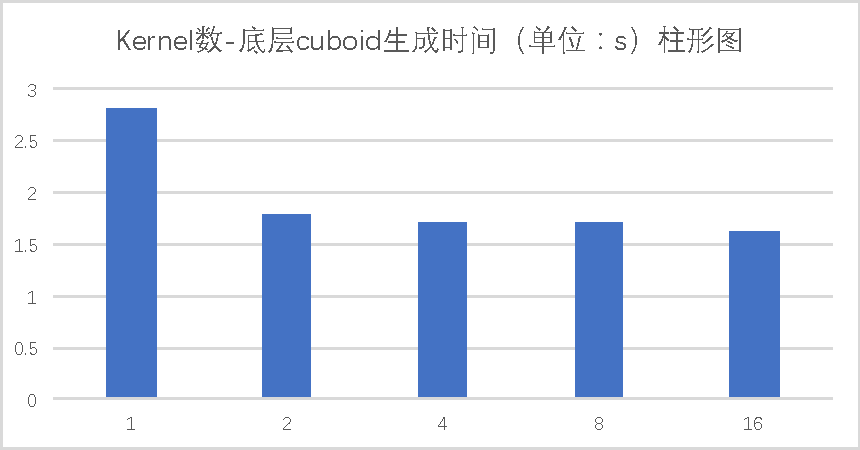
\includegraphics{CPU-KernelNumber-cuboidGenerate}
\caption{CPU:Kernel数-底层cuboid生成时间(单位:s)柱形图} 
\label{fig:figure1}
\end{figure}

另外,对于不同规模的数据集的测试有结果如下(基于kernel数=16)

\begin{table}[!htbp]
\centering
\caption{CPU:数据集大小-底层cuboid生成时间(单位:s)表} 
\label{tab:table5}
\begin{tabular}{|c|c|}
    \hline
    数据集条目数 & 计算部分的运行时间(s)\\
    \hline
    262144 & 0.0260788\\
    \hline
    2097152 & 0.06733256\\
    \hline
    16777216 & 0.3991288\\
    \hline
    134217728 & 1.62508\\
    \hline
\end{tabular}
% \note{这里是表的注释}
\end{table}

\begin{figure}[ht]
\centering
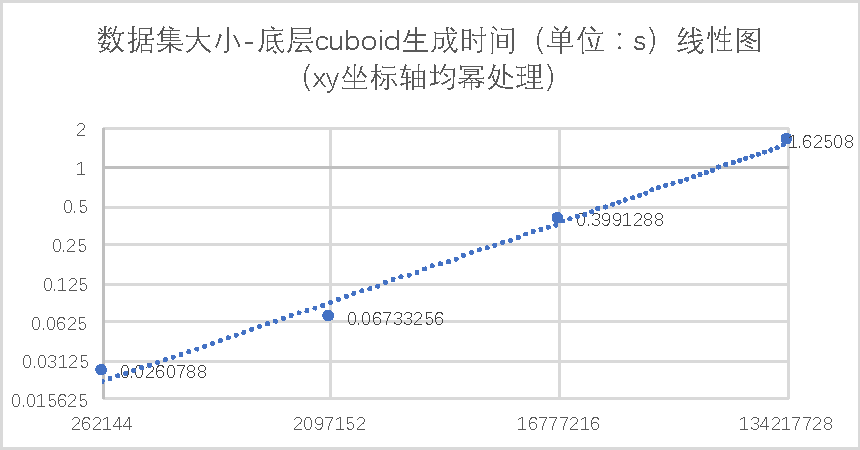
\includegraphics{CPU-DatasetSize-cuboidGenerate}
\caption{CPU:数据集大小-底层cuboid生成时间(单位:s)线性图} 
\label{fig:figure2}
\note{$x$, $y$轴均经过了幂处理}
\end{figure}

在不同的kernel运行时,从系统管理中能够查询到的内存空间占用如下表:

\begin{table}[htbp]
\centering
\caption{CPU:数据集大小-kernel数-内存占用(单位:MB)表} 
\label{tab:table6}
\begin{tabular}{|c|c|c|}
    \hline
    数据集条目数 & kernel数 & 总内存占用\\
    \hline
    262144 & 1 & 18.5\\
    \hline
    262144 & 2 & 25.0\\
    \hline
    262144 & 4 & 37.9\\
    \hline
    262144 & 8 & 63.8\\
    \hline
    262144 & 16 & 115.6\\
    \hline
    2097512 & 16 & 171.6\\
    \hline
    16777216 & 16 & 619.6\\
    \hline
\end{tabular}
% \note{这里是表的注释}
\end{table}

由上面这些测试数据和图表,可以得到如下结论:

1、由于该实验平台的CPU是$2$ core的,因此在多核实验中,生成的计算核心在超过$2$之后运行速度并没有实质性的变化(因为系统同时只能执行两个计算核心)。

2、另一方面,通过数据集大小和生成底层cuboid的时间的图表,可以看到这个算法运行的时间确实和原始数据集大小基本呈线性关系,与最初的算法分析一致。

在CPU-GPU架构上:

为了检验算法在更多核的平台上是否具有更好的可拓展性,因此该实验在GPU上重新部署了一遍。采用的数据集是$16777216$条目的数据集。具体的实验结果如下所示,其中所有的测量值都是五次测量的平均数。

\begin{table}[!htbp]
\centering
\caption{GPU:Kernel数-底层cuboid生成时间(单位:s)表} 
\label{tab:table7}
\begin{tabular}{|c|c|}
    \hline
    kernel数 & 计算部分的运行时间(s)\\
    \hline
    12 & 7.503698\\
    \hline
    16 & 6.260434\\
    \hline
    32 & 3.76185\\
    \hline
    48 & 2.971528\\
    \hline
    64 & 2.967586\\
    \hline
\end{tabular}
% \note{这里是表的注释}
\end{table}

\begin{figure}[ht]
\centering
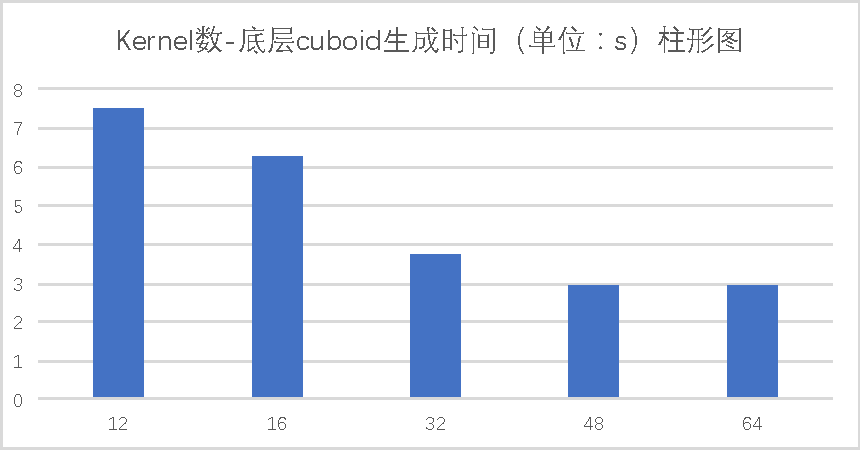
\includegraphics{GPU-KernelNumber-cuboidGenerate}
\caption{GPU:Kernel数-底层cuboid生成时间(单位:s)柱形图} 
\label{fig:figure3}
\end{figure}

由此可见,虽然实验结果的数值受限于硬件,仍然可以看出该并行算法具有很好的可拓展性,在具有更多(流)处理核心的并行计算平台上将获得更大的收益。

\subsection{对于由cuboid到cuboid的聚合算法的评估}

这一小节中将进行有无采用并行方式对于聚合性能的评估

在纯CPU架构上:

在本部分的测试中,我们将固定在cuboid聚合中使用聚合路线选择算法。采用的原始cuboid是基于$262144$个元素的数据集生成的cell总数为$24947$$(19, 101, 13)$的cuboid,目标cuboid是三步聚合后的顶层cuboid。另外,所有测试均采用下文将要测试的聚合路径优化算法。
测试结果如下:

\begin{table}[!htbp]
\centering
\caption{CPU:Kernel数-从cuboid到cuboid聚合时间(单位:s)表} 
\label{tab:table8}
\begin{tabular}{|c|c|}
    \hline
    kernel数 & 计算部分的运行时间(s)\\
    \hline
    1 & 0.001860436\\
    \hline
    2 & 0.001092724\\
    \hline
    4 & 0.00081602\\
    \hline
    8 & 0.000845582\\
    \hline
\end{tabular}
% \note{这里是表的注释}
\end{table}

\begin{figure}[ht]
\centering
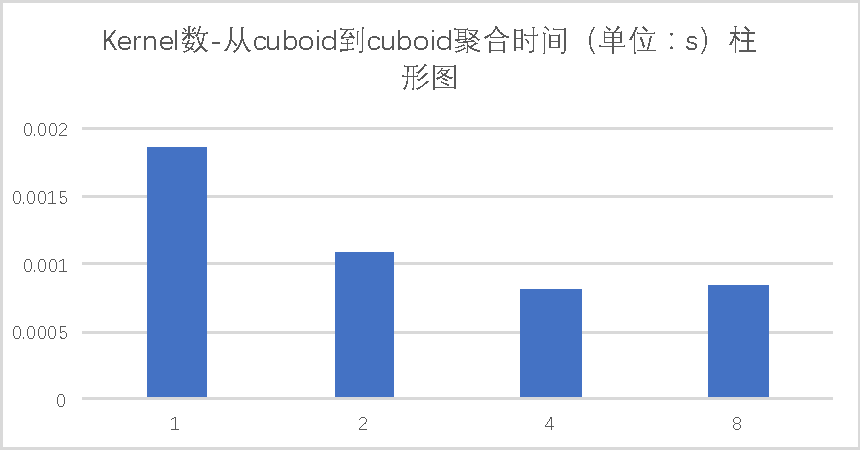
\includegraphics{CPU-KernelNumber-fromto}
\caption{CPU:Kernel数-从cuboid到cuboid聚合时间(单位:s)柱形图} 
\label{fig:figure4}
\end{figure}

在CPU-GPU架构上:
相同于之前的测试,这里我们仍然使用如下测试方法:原始cuboid是基于$262144$个元素的数据集生成的cell总数为$24947$$(19, 101, 13)$的cuboid,目标cuboid是三步聚合后的顶层cuboid。另外,所有测试均采用下文将要测试的聚合路径优化算法。
测试结果如下:

\begin{table}[!htbp]
\centering
\caption{GPU:Kernel数-从cuboid到cuboid聚合时间(单位:s)表} 
\label{tab:table9}
\begin{tabular}{|c|c|}
    \hline
    kernel数 & 计算部分的运行时间(s)\\
    \hline
    12 & 0.044490438\\
    \hline
    16 & 0.036521843\\
    \hline
    32 & 0.024351568\\
    \hline
    64 & 0.015527524\\
    \hline
\end{tabular}
% \note{这里是表的注释}
\end{table}

\begin{figure}[ht]
\centering
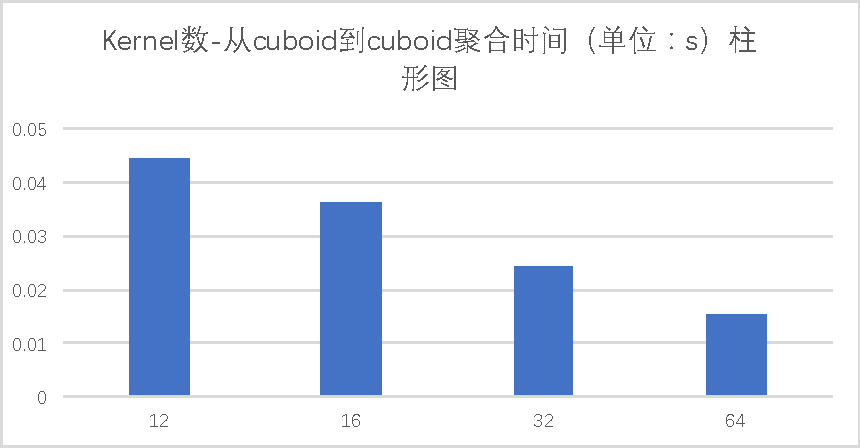
\includegraphics{GPU-KernelNumber-fromto}
\caption{GPU:Kernel数-从cuboid到cuboid聚合时间(单位:s)柱形图} 
\label{fig:figure5}
\end{figure}

从上述两组测量数据中也能够看出,并行之后的算法效率比起未并行之时有了很大的提升。另外,并行算法的良好的可扩展性也在实验数据中有所体现:其他条件相同的前提下,更高的并行数会带来更高的执行效率。

\subsection{对于聚合路线选择算法的评估}

在本小节中,我们将测试不同的聚合路线选择对于从一个较原始的cuboid到另一个上游cuboid的聚合性能的影响。

下文将列出参加测试的原始cuboid的各项参数,以及实际程序运行的结果。为了控制变量的原则,这里固定采用的硬件是CPU,OpenCL生成的计算kernel数为$16$。这些原始cuboid都是在之前的实中中生成的。为了简单起见,我们假定所有的聚合的最终目标都是一个“全维度聚合”cuboid,即一个顶层cuboid,从它将无法再进行任何聚合。

\begin{table}[!htbp]
\centering
\caption{CPU:聚合路径的选择与否系列图表(单位:s)表} 
\label{tab:table10}
\begin{tabular}{|c|c|c|c|c|c|}
    \hline
    原数据集条目数 & cell个数 & 路径优化 & 第一步 & 第二步 & 第三步\\
    \hline
    134217728 & 24947 & T & 0.00085184 & 0.00002840 & 0.00000615\\
    \hline
    134217728 & 24947 & F & 0.00082885 & 0.00010397 & 0.00001860\\
    \hline
    262144 & 24947 & T & 0.00085994 & 0.00002619 & 0.00000640\\
    \hline
    262144 & 24947 & F & 0.00083391 & 0.00016831 & 0.00001782\\
    \hline
    262144 & 3333 & T & 0.00027702 & 0.00000758 & 0.00000573\\
    \hline
    262144 & 3333 & F & 0.00026012 & 0.00004609 & 0.00002158\\
    \hline
\end{tabular}
% \note{这里是表的注释}
\end{table}

根据测试所得数据,可以做出柱形图来表现出各种不同的对比方式之间的性能差异。

\begin{figure}[ht]
\centering
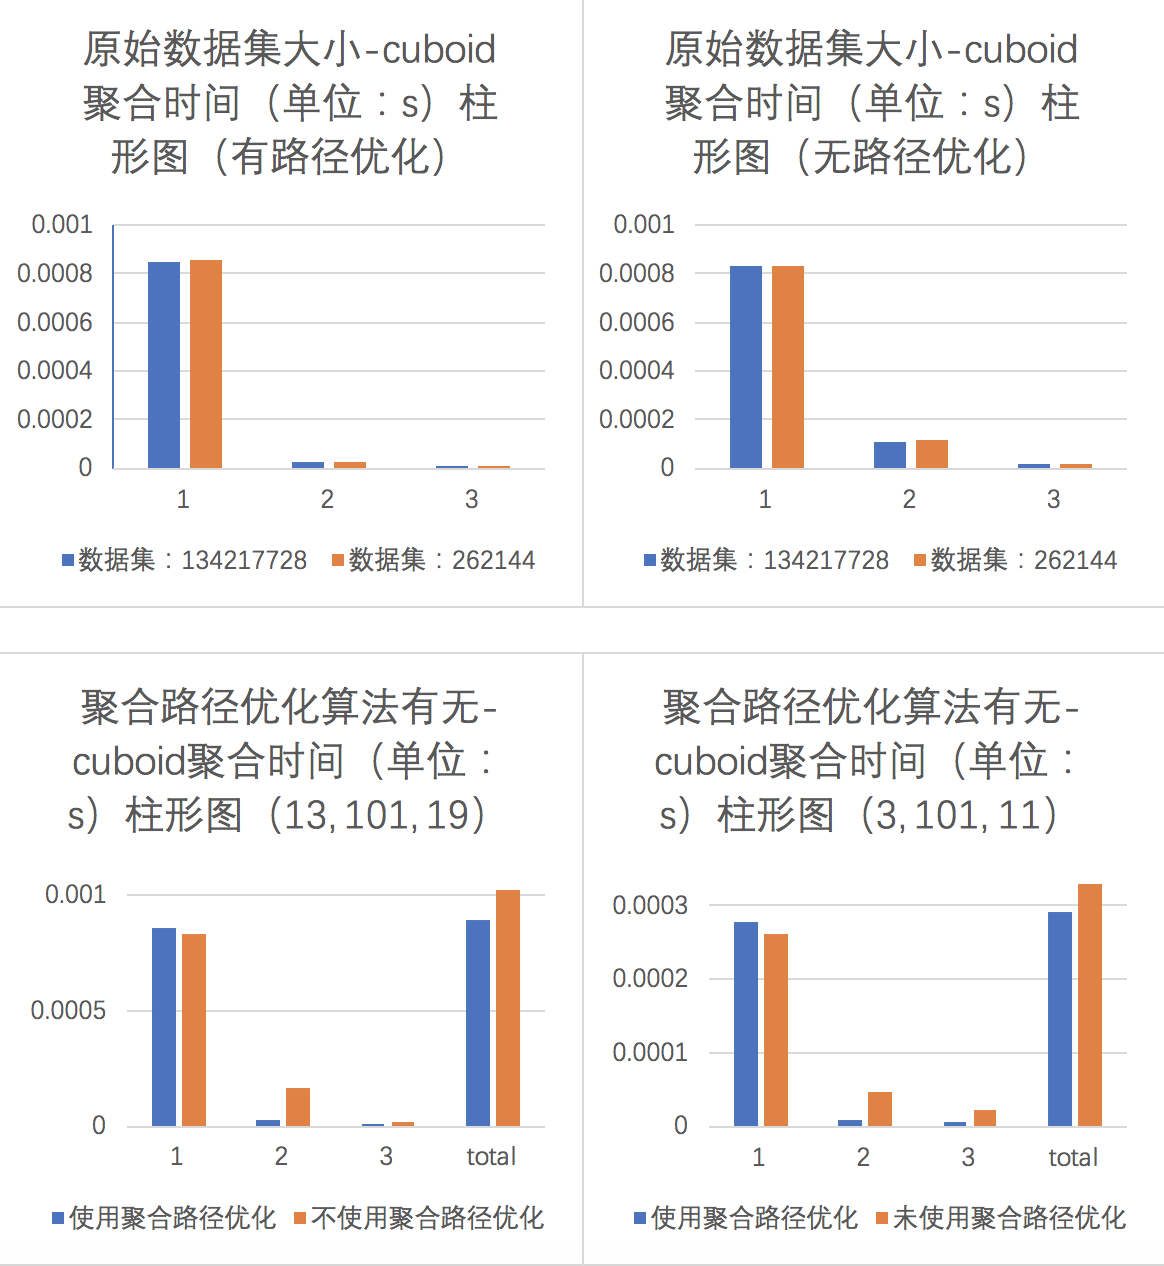
\includegraphics[width=10cm]{CPU-aggregateroute}
\caption{CPU:聚合路径的选择与否系列图表(单位:s)柱形图} 
\label{fig:figure6}
\end{figure}

可以从数据汇总表格和柱形图中看到如下规律:

1、由于这个算法是从cuboid出发的计算算法,因此与原始数据集的大小无关。

2、如同分析的那样,我们的路径优化算法在第一步聚合时是不会起到任何作用的,因此第一步的执行时间基本相同,可能由于系统架构或者是代码书写的问题,使用路径优化的方案甚至略慢于不使用路径优化的方案。而从第二步开始,经过了聚合路径优化的算法开始凌驾于未经过优化的算法。但是由于第一步聚合占用的时间占了整个聚合步骤的最主要部分,因此总体时间上来看优化的比例大概在10\%-15\%之间。

\subsection{花费函数在不同实验平台上的实际计算}

根据前文测试所得结果,下面我们分别在不同的平台上计算出一个花费函数,并且用这个花费函数与Stanford的方案下的花费函数来计算在不同情形下的预处理集合,以及评估他们之间的性能差距。

这个测试中,由于本身维度空间比较小(共$3$个维度),所以可能的cuboid总数$2^3 = 8$也并不是太多,因此在我们的测试中固定预处理的cuboid数量为$2$。评估最后的性能时,我们将以“除去底层cuboid以外的所有$7$个cuboid生成的总时间”作为评估标准。我们采用的底层cuboid的总cell数为$24947$,其中三个维度的值分别为$(19, 101, 13)$。另外,我们此处固定采用聚合路径优化算法。

在纯CPU架构上:

根据之前小节中估计的结果,我们已经有了花费函数估计式中的三个系数如下:

$C_{copy\_hd\_to\_m} = 9.34613 \times 10^{-8}$s / byte

$C_{init\_time} = 0.00225$s

$C_{copy\_d\_to\_m} = C_{copy\_m\_to\_d} = 4.70919 \times 10^{-10}$s / byte

考察$t_{scan\_per\_cell}$,其指的是在从cuboid到cuboid聚合时“单个kernel”对于“聚合前的单个cell”的处理时间。因此,这个地方要进行计算时,首先要选择的数据集应该也是“单kernel前提下”进行聚合的时间测量结果。因此我们将采用之前小节中聚合cuboid的测量数据进行计算。

测量表格中,给出的是“三步聚合的时间总和”,实际上我们在测量时也测量了第一步聚合的时间。我们在这里选择第一步聚合的时间作为我们的计算基准,是因为这样能尽可能平摊可能产生的系统与测量误差到每一个cell上,从而让我们的估计更为精确。

从实验数据中我们可以直接得到,在该平台上,对于$24947$个cell的扫描/聚合操作的总时间为$0.00184109$s,即$t_{scan\_per\_cell} = 0.00184109 \div 24947 = 7.38 \times 10^{-8}$s / cell

在CPU-GPU架构上:

根据之前小节中估计的结果,我们已经有了花费函数估计式中的三个系数如下:

$C_{copy\_hd\_to\_m} = 1.26069 \times 10^{-8}$s / byte

$C_{init\_time} = 0.195$s

$C_{copy\_d\_to\_m} = C_{copy\_m\_to\_d} = 1.7 \times 10^{-14}$s / byte

利用与之前类似的方法,也能计算出$t_{scan\_per\_cell} = 1.36165 \times 10^{-5}$s / cell

考察上一章中花费函数中提到的$count_A$与$count_B$,结合我们此处具体设置的实验条件,我们可以直接给出关于这两个量在所有情况下的具体取值。此时“cell的处理个数”指的是由原始cuboid到目标cuboid的路径上总共需要处理的cell个数。

\begin{table}[!htbp]
\centering
\caption{$count_A$表} 
\label{tab:table11}
\begin{tabular}{|l|l|}
    \hline
    目标cuboid的cell个数 & $count_A$(总共需处理的cell个数)\\
    \hline
    1919 & 24947\\
    \hline
    1313 & 24947\\
    \hline
    247 & 24947\\
    \hline
    101 & 24947 + 1313 = 26260\\
    \hline
    19 & 24947 + 247 = 25194\\
    \hline
    13 & 24947 + 247 = 25194\\
    \hline
    1 & 24947 + 247 + 13 = 25207\\
    \hline
\end{tabular}
% \note{这里是表的注释}
\end{table}

\begin{table}[!htbp]
\centering
\caption{$count_B$表} 
\label{tab:table12}
\begin{tabular}{|l|l|}
    \hline
    目标cuboid的cell个数 & $count_B$(总共需处理的cell个数)\\
    \hline
    1919 & 1919\\
    \hline
    1313 & 1313\\
    \hline
    247 & 247\\
    \hline
    101 & 1313 + 101 = 1414\\
    \hline
    19 & 247 + 19 = 266\\
    \hline
    13 & 247 + 13 = 260\\
    \hline
    1 & 247 + 13 + 1 = 261\\
    \hline
\end{tabular}
% \note{这里是表的注释}
\end{table}

于是,根据以上这些数据,我们可以计算出在两个不同的平台上的所有cuboid的$C(v)$了。

首先针对通常的database system,这样的system将预处理的cuboid缓存在硬盘等外部存储设备中。下面两个表格给出了我们计算出的$C(v)$值。第一列如同前述两个count的表格,均指的目标cuboid中的cell个数;第二列则直接列出根据前述花费函数公式,以及本小节中给出的常数值来计算的每个cuboid的花费值。

在纯CPU平台上:

\begin{table}[!htbp]
\centering
\caption{CPU + HD平台上的cell个数-$C(v)$表} 
\label{tab:table13}
\begin{tabular}{|l|l|}
    \hline
    将预处理cuboid的cell个数 & $C(v)$\\
    \hline
    1919 & -0.234726\\
    \hline
    1313 & -0.240735\\
    \hline
    247 & -0.251306\\
    \hline
    101 & -0.252971\\
    \hline
    19 & -0.253608\\
    \hline
    13 & -0.253666\\
    \hline
    1 & -0.253789\\
    \hline
\end{tabular}
% \note{这里是表的注释}
\end{table}

在CPU-GPU平台上:

\begin{table}[!htbp]
\centering
\caption{GPU + HD平台上的cell个数-$C(v)$表} 
\label{tab:table14}
\begin{tabular}{|l|l|}
    \hline
    将预处理cuboid的cell个数 & $C(v)$\\
    \hline
    1919 & -0.247233\\
    \hline
    1313 & -0.248049\\
    \hline
    247 & -0.249484\\
    \hline
    101 & -0.250798\\
    \hline
    19 & -0.250001\\
    \hline
    13 & -0.250009\\
    \hline
    1 & -0.250036\\
    \hline
\end{tabular}
% \note{这里是表的注释}
\end{table}

可以看出来,在我们的估计方案的基础上估计出来的$C(v)$和传统Stanford方案估计出来的不一样:并非按照cell个数而单调递增。

然后,在计算出来的$C(v)$值的基础上,我们会发现,实际上我们得到的$S$集合是一样的。这证明了我们的方案至少不会比Stanford原有的方案更差。具体关于这部分的原因会在接下来的小节中提到。

我们使用预处理的方案与未预处理的方案进行比对,能得到如下结果(运行在CPU平台上):

\begin{table}[!htbp]
\centering
\caption{CPU:预处理-全cuboid生成时间(单位:s)表} 
\label{tab:table15}
\begin{tabular}{|c|c|c|}
    \hline
    处理方式 & 预处理 & 未预处理\\
    \hline
    时间总和(读取文件+处理) & 0.289799 & 0.901132\\
    \hline
\end{tabular}
% \note{这里是表的注释}
\end{table}

\begin{figure}[ht]
\centering
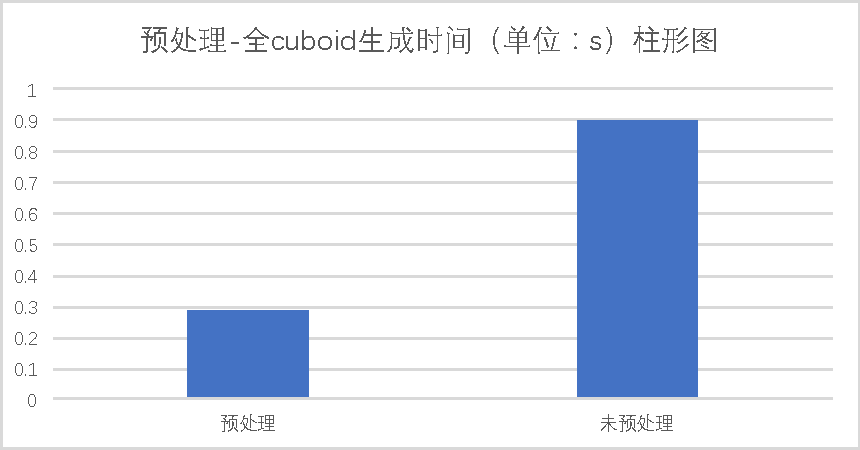
\includegraphics{CPU-preprocessing}
\caption{CPU:预处理-全cuboid生成时间(单位:s)柱形图} 
\label{fig:figure7}
\end{figure}

可以看到,进行了两次预处理之后,最占用运行时间的次低层cuboid的生成都被免去了,从而使得运行效率大幅度提高了。

接下来针对in-memory database模型,这样的database system会将尽可能多的有用信息缓存在memory中,从而使得对这部分数据的读写效率大幅提升。

首先计算这个前提下的$C(v)$。由于假定预处理完毕的cuboid现在存放在内存中,因此我们采用4.4.2.后半段提出来的适用于该情形的花费函数。该花费函数中没有$C_{copy\_hd\_to\_m}$一项。

以下是在该前提下计算出来的新的$C(v)$

在纯CPU平台上:

\begin{table}[!htbp]
\centering
\caption{CPU + in-memory平台上的cell个数-$C(v)$表} 
\label{tab:table16}
\begin{tabular}{|l|l|}
    \hline
    将预处理cuboid的cell个数 & $C(v)$\\
    \hline
    1919 & -0.00489118\\
    \hline
    1313 & -0.00485236\\
    \hline
    247 & -0.00478409\\
    \hline
    101 & -0.00499137\\
    \hline
    19 & -0.00481024\\
    \hline
    13 & -0.00480986\\
    \hline
    1 & -0.00481124\\
    \hline
\end{tabular}
% \note{这里是表的注释}
\end{table}

在CPU-GPU平台上:

\begin{table}[!htbp]
\centering
\caption{GPU + in-memory平台上的cell个数-$C(v)$表} 
\label{tab:table17}
\begin{tabular}{|l|l|}
    \hline
    将预处理cuboid的cell个数 & $C(v)$\\
    \hline
    1919 & -0.2162307387\\
    \hline
    1313 & -0.2162307373\\
    \hline
    247 & -0.2162307348\\
    \hline
    101 & -0.2173481446\\
    \hline
    19 & -0.21644094018\\
    \hline
    13 & -0.21644094016\\
    \hline
    1 & -0.2164520036\\
    \hline
\end{tabular}
% \note{这里是表的注释}
\end{table}

此时我们可以发现,$C(v)$的生成方式已经和Stanford有了很大的区别。在这个基础上计算出来的$S$集合如下:

Stanford:${24947, 247, 1313}$

我们的方案\_纯CPU:${24947, 1919, 1313}$

我们的方案\_CPU-GPU:(同上)

这里也能看出来,在CPU-GPU平台上,去掉了$C_{copy\_hd\_to\_m}$项之后,由于$C_{copy\_m\_to\_d}$项对$t_{scan\_per\_cell}$项影响实在微乎其微,因此整个式子的相对大小关系基本全部由扫描一项决定,即扫描的cuboid数($count_A$表)成为了$C(v)$差异的关键。而事实上由$count_A$表中也能看出来,由于聚合路径选择算法,使得后续步数的聚合远比前面一步的扫描要耗时更少,因此扫描的cuboid数量几乎没有差距,所以最终体现出来估计值几乎完全相同的情况。

最后,我们使用算法给出的预处理集合,分别测试两种预处理方案的性能差距。结果如下(运行在CPU平台上):

\begin{table}[!htbp]
\centering
\caption{CPU:预处理方式-全cuboid生成时间(单位:s)表} 
\label{tab:table18}
\begin{tabular}{|c|c|c|}
    \hline
    处理方式 & 我们的方式 & Stanford\\
    \hline
    时间总和(仅处理) & 0.00081504 & 0.00087807\\
    \hline
\end{tabular}
\note{在我们对in-memory模型的假定中,不存在硬盘读写}
\end{table}

\begin{figure}[ht]
\centering
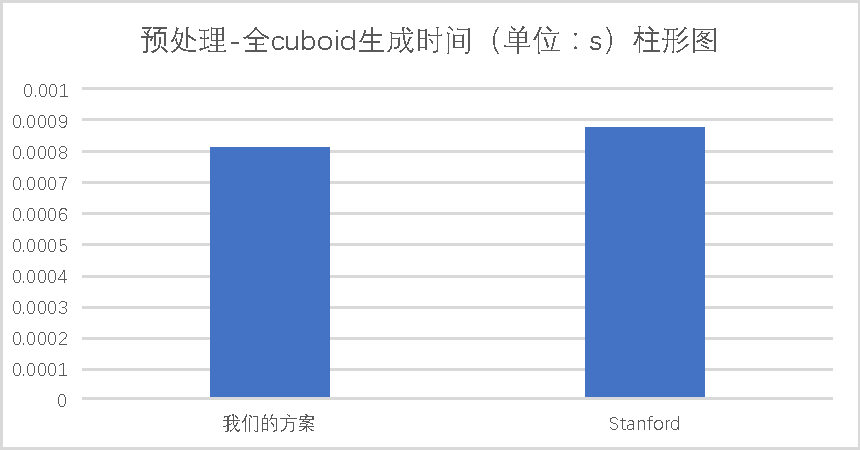
\includegraphics{CPU-preprocessing-approach}
\caption{CPU:预处理方式-全cuboid生成时间(单位:s)柱形图} 
\label{fig:figure8}
\end{figure}

可以看到,虽然差距不很明显,但是在这个场景设置下我们的预处理方案略优于Stanford提出的方案。

\section{实验分析与讨论}

\subsection{何时使用生成并行化的数据立方体生成的混合方案的考量}
在本小节中,我们将考察何时必须采用混合方案。

显然,若是条件允许,速度最优方案易于内存管理,易于程序流程控制并且拥有最高的运行速度,应该是我们的首选。而也如前所述,速度最优方案中的最大的问题在于潜在的占用内存空间过多问题。因此考察混合方案何时必须被使用,其实另一方面来说也是考察速度最优方案使用的边界条件。

在讨论内存空间问题的大前提下,我们可以发现,在整个算法运行之中,占用内存最多的主要是两块数据:直接读入的原始数据集,以及在运行中产生的临时subcuboid。下面就从这两个方面来分析其对于方案选择的影响。

在前面的的实验数据中,可以计算得出,在本实验所给定的cell的结构基础上,一个拥有$24947$个cell的cuboid所占用的空间约为$6.5$MB。因此仅从设备空间因素考虑,假定我们有$2$GB内存空间能够分配给这些临时subcuboid的前提下,能够同时运行的最大kernel数和一个cuboid的总cell数的关系大概如下:

\begin{table}[!htbp]
\centering
\caption{cell数目-最大可同时生成kernel数表} 
\label{tab:table19}
\begin{tabular}{|c|c|c|}
    \hline
    cuboid的cell的个数 & 最大可同时生成kernel数 & CPU or GPU\\
    \hline
    1000 & 7692 & GPU\\
    \hline
    5000 & 1538 & GPU\\
    \hline
    10000 & 769 & GPU\\
    \hline
    25000 & 307 & GPU\\
    \hline
    50000 & 153 & GPU\\
    \hline
    100000 & 76 & maybe GPU\\
    \hline
    250000 & 30 & maybe very good CPU\\
    \hline
    1000000 & 15 & CPU\\
    \hline
    2500000 & 6 & CPU\\
    \hline
    5000000 & 3 & CPU\\
    \hline
    7500000 & 1 & x\\
    \hline
\end{tabular}
\note{在我们对in-memory模型的假定中,不存在硬盘读写}
\end{table}

基本可以得到如下结论:在维度总乘积小于$100000$的时候,基本上可以不做任何调整将其部署在GPU上进行并行计算,正如本论文中实验所涉及到的数据集那样。在$100000$~$2500000$的区间,如果为了保证在GPU上的并行度,则应该转而采取混合方案来进行计算;而在CPU上仍可以采用直接计算的方法而不影响到并行度。在更大的区间上,则由于存储空间已经不足以支持数个,甚至是一个完整的cuboid,则无论CPU抑或是GPU都应该采取混合方案来进行计算。

然后,我们再来考察一下数据集大小对于是否采用混合方案的影响。然而实际上,由于本来就存在“原始数据集过大以至于无法一次全部读取”的问题,所以在内存的分配上,我们可以主要以cuboid占用的总空间作为衡量标准,然后对原dataset进行一定程度的划分,使得每个part的内存占用与临时subcuboid占用的空间总和不超过允许的最大限度。在此基础上,每次都在其中的一个part上运行我们的算法(然后我们的算法在运行过程中把这个part再分成一些更小的part),并将这个part的聚合结果暂时存储在一些其他存储介质中,最后再收集起来形成一个完整的数据集的底层cuboid。

综合以上两部分的分析,我们可以得知,采取何种方案其实直接相关于问题的规模,即我们需要得到的cuboid具体的cell总数的多少。然后在这个基础上,我们可以适当的在编程上对一次读入的数据集的大小进行调整,使得程序能尽可能更快地运行。

\subsection{对于修正后的花费函数的评估}

在本小节中,我们主要评估在不同的实验平台,也就是在不同的系数修正下得到的我们的估计花费函数和Stanford方案的差异点。

可以发现,实际上在硬盘性能不足,抑或是并行执行的算法计算量本身并非太大的话,对应项的系数修正之后,我们的方案的花费函数的最终表达式基本上和Stanford的式子是统一的:修正系数能让我们的花费函数的读写时间项的影响和别的项有超过1个数量级的差距,甚至更大。

而当我们在更宽的主板数据总线/更快的硬盘,或者直接忽略从外部存储到主存的时间(in-memory mode),抑或是运行更复杂的,计算量更大的并行算法的时候,系数的修正有时就会使得修正后的花费函数开始偏向于花费函数中的计算项或者是设备之间的拷贝项。此时两种花费函数所选择出来的预处理cuboid将有可能有所区别。而因为我们的花费函数直接以时间作为考量因素,因此在以时间作为衡量标准的最终运行效率上比以空间作为运行效率的间接考量因素的Stanford方案不会更差。

但无论怎样,我们的方案指出了一个事实:在不同的硬件平台,不同的算法构成的前提下,花费函数都是需要重新计算的。

